\chapter{Diagramma delle classi}

\section{Definizione delle classi}

    \subsection*{1. Utente}
        La classe ``Utente'', da cui la classe omonima, rappresenta la classe astratta che viene estesa da tutte le tipologie di utenti presenti all'interno del programma. All'interno della classe Utente sono presenti i campi contenenti le informazioni personali ed i metodi comuni a tutti gli utenti, oppure necessari per definire il ruolo che l'utente ricopre all'interno del programma stesso.

    \subsection*{2. Utente\_Analista}
        La classe ``Utente\_Analista'' rappresenta la classe di utenti che hanno la possibilità di visualizzare una maggiore quantità di informazioni e di statistiche al fine di analizzarne l'andamento e di studiare le strategie più efficaci per aumentare il grado di soddisfazione dei cittadini all'interno della città. La classe estende la classe ``Utente'', alla quale aggiunge gli attributi e i metodi necessari per gestire l'area di influenza dell'Analista stesso.

    \subsection*{3. Utente\_Sondaggista}
        La classe ``Utente\_Sondaggista'' raffigura la classe di utenti che hanno la possibilità di aggiungere o eliminare i sondaggi ed i voti presenti all'interno dei sondaggi stessi, permettendo ai cittadini la possibilità di esprimere il proprio grado di soddisfazione riguardo i servizi comunali e le politiche attutate dal comune. La classe estende la classe ``Utente'', alla quale aggiunge gli attributi e i metodi necessari per gestire i sondaggi, i voti e l'area di influenza del sondaggista stesso.

    \subsection*{4. Utente\_Circoscrizione}
        La classe ``Utente\_Circoscrizione'' raffigura la classe di utenti che hanno la possibilità di gestire le funzionalità di maggiore rilievo all'interno della circoscrizione di appartenenza, tra le quali la gestione delle strutture, dei ruoli e delle richieste. La classe estende la classe ``Utente'', alla quale aggiunge gli attributi e i metodi necessari per le funzionalità di gestione delle strutture, dei ruoli e delle richieste.

    \subsection*{5. Utente\_Amministratore}
        La classe ``Utente\_Amministratore'' raffigura la classe di utenti che hanno la possibilità di gestire le funzionalitàdi maggiore rilievo all'interno del comune di appartenenza, tra le quali la gestione delle strutture, dei ruoli e delle richieste. La classe estende la classe ``Utente'', alla quale aggiunge gli attributi e i metodi necessari per le funzionalità di gestione delle strutture, dei ruoli e delle richieste.

    


\section{Diagramma delle classi complessivo}
    Riportiamo di seguito il diagramma delle classi con tutte le classi fino ad ora presentate.
    \begin{figure}[H]
        \centering
        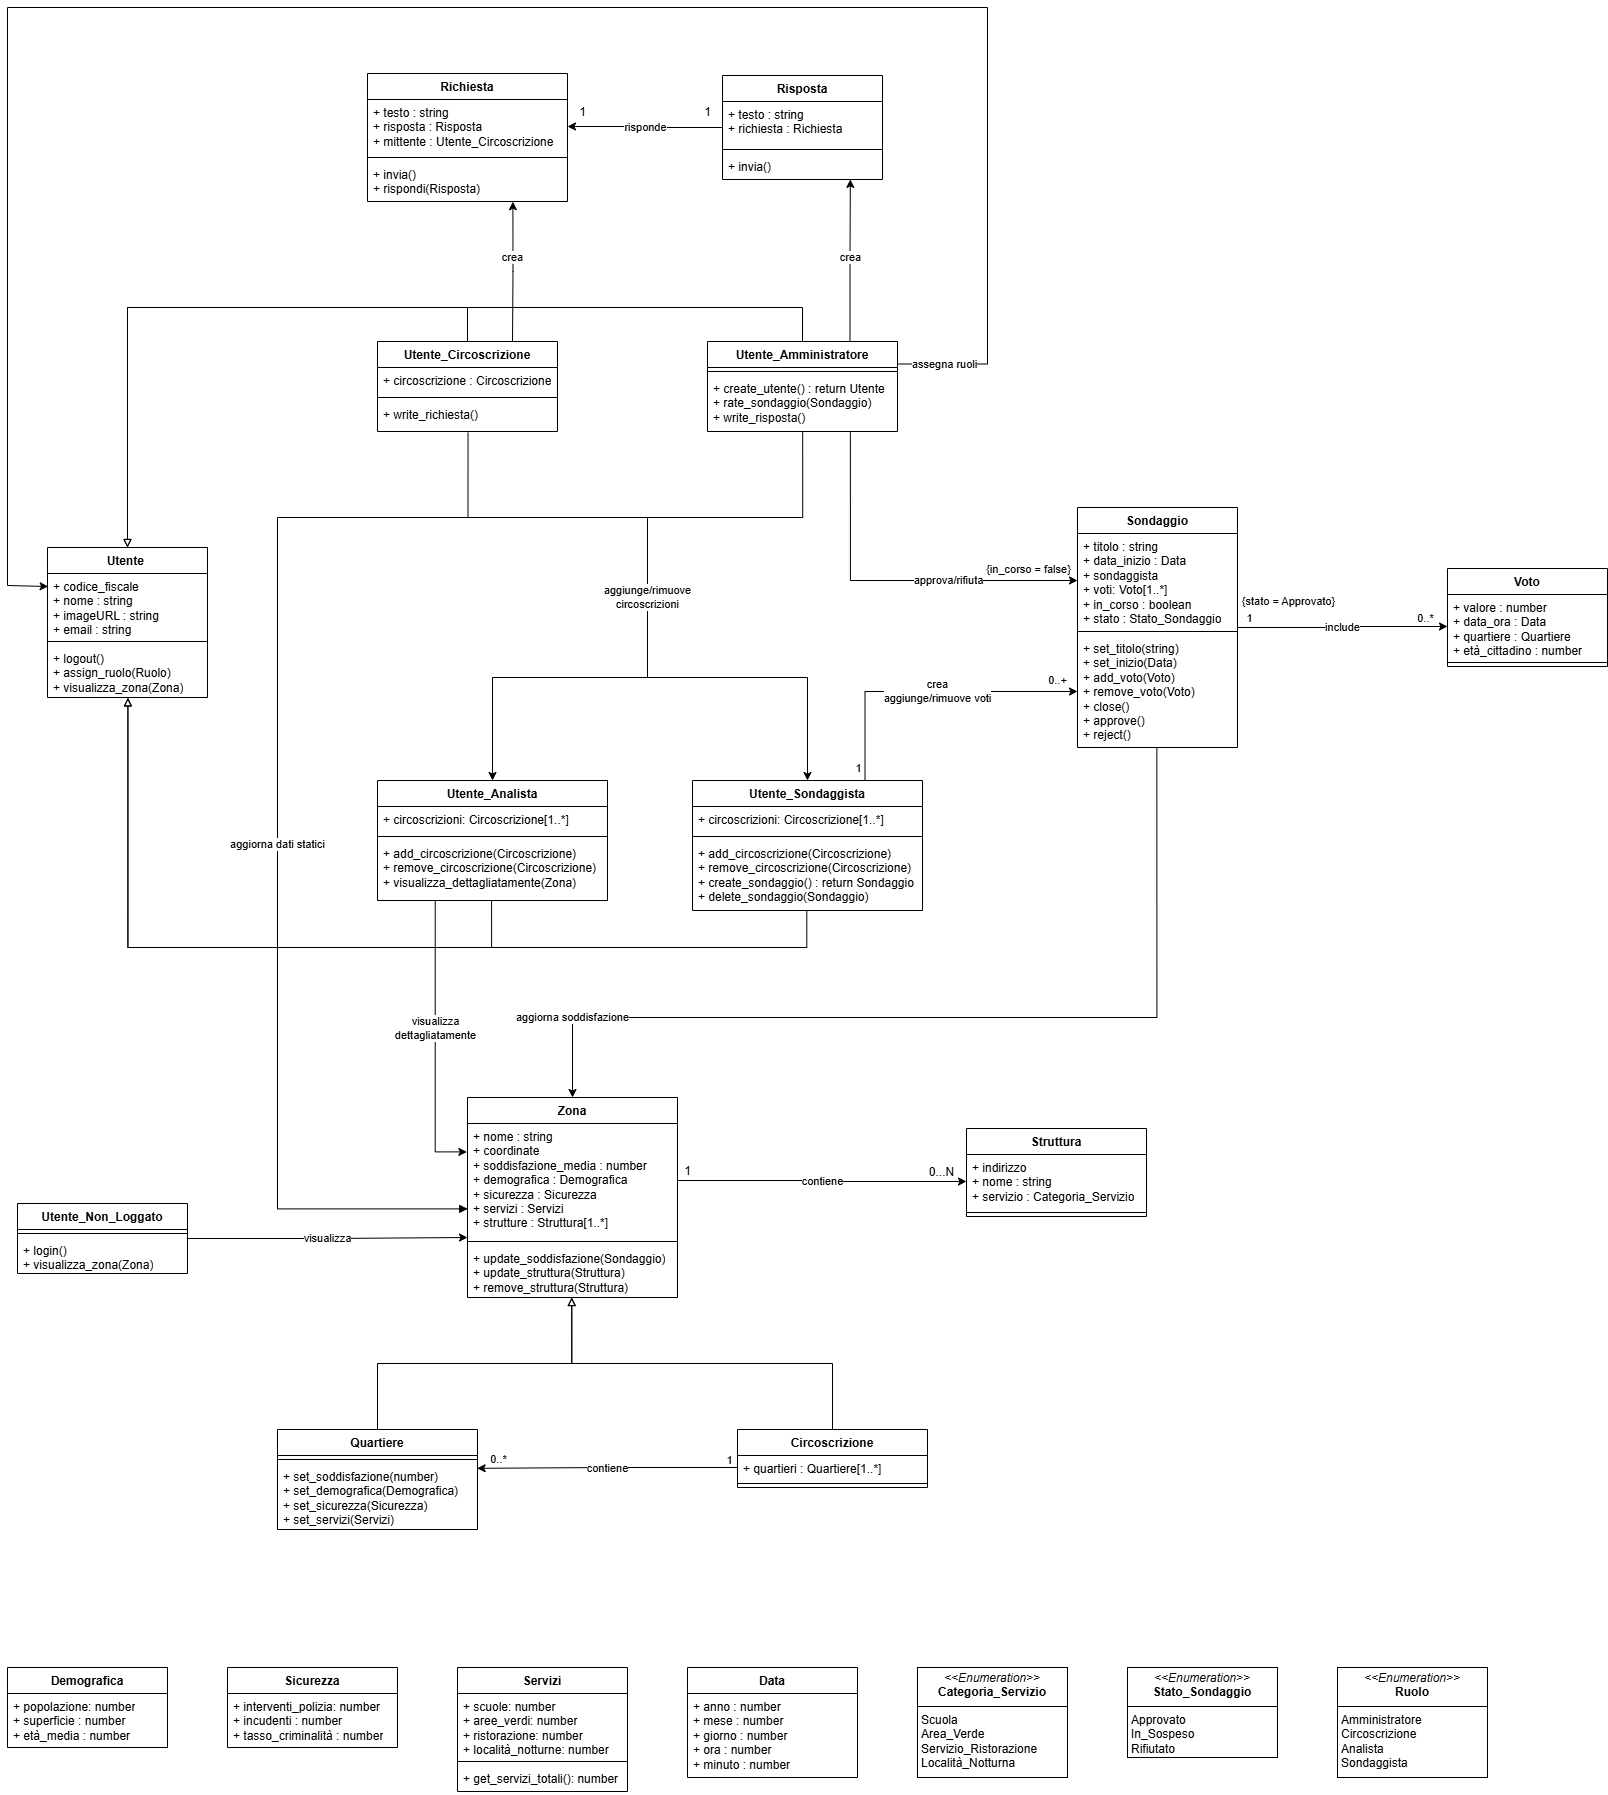
\includegraphics[width=1\textwidth]{ClassDiagram/ClassDiagram.drawio.png}
    \end{figure}